\documentclass{beamer}
\usepackage[]{cb-style}
\usepackage{animate}
\usepackage{subfig}

\newcommand{\IR}{{\mathbb R}}
\newcommand{\IC}{{\mathbb C}}
\newcommand{\IN}{{\mathbb N}}
\newcommand{\IZ}{{\mathbb Z}}
\newcommand{\bx}{{\mathbf x}}
\newcommand{\bd}{{\mathbf d}}
\newcommand{\bn}{{\mathbf n}}
\newcommand{\bE}{{\mathbf E}}

\newcommand{\inc}{{\mathrm{inc}}}
\newcommand{\tot}{{\mathrm{tot}}}
\newcommand{\scat}{{\mathrm{scat}}}
\newcommand{\ri}{{\mathrm i}}
\newcommand{\re}{{\mathrm e}}
\newcommand{\rd}{{\,\mathrm d}}

\begin{document}
	
	\begin{frame}{}
		\tableofcontents
	\end{frame}
	
	\section{Equazione di Helmholtz}
	\sectionpage
	
	\begin{frame}{Perché l'equazione di Helmholtz?}
		\begin{small}
		Sia $U=U(\bx,t)$ un campo scalare. Supponiamo che $U$ soddisfi l'\textbf{equazione delle onde}
		\begin{equation*}
			\frac{1}{c^2} \frac{\partial^2U}{\partial t^2} - \Delta U = 0.
		\end{equation*}
		Consideriamo il caso particolare di una soluzione \textbf{armonica in tempo}
		\begin{equation*}
			U(\bx,t) = \Re \{ u(\bx)\re^{-\ri\omega t}\} = \Re \{u(\bx)\} \cos \omega t + \Im \{u(\bx)\} \sin \omega t,
		\end{equation*}
		per una certa \textbf{frequenza angolare} $\omega>0$. Si ottiene il seguente fatto fondamentale
		\begin{block}{}
			Se $U(\bx,t)$ è una soluzione delle onde armonica in tempo, allora $u(\bx)$ è soluzione dell'\textbf{equazione di Helmholtz}
			\begin{equation*}
				\Delta u + k^2u = 0,
			\end{equation*}
			con \textbf{numero d'onda} $k:= \omega/c>0$.
		\end{block}
		\end{small}
	\end{frame}
	
	
	\begin{frame}{Soluzioni particolari dell'equazione di Helmholtz}
		\begin{small}
		 \begin{block}{Onde piane}
		 	Dato $\bd \in \IR^2$, un'\textbf{onda piana} che si propaga lungo la direzione $\bd$ ha espressione \begin{equation*}
		 		u(\bx) = \re^{\ri k \bx \cdot \bd} = \cos(k\bx \cdot \bd)+\ri\sin(k\bx \cdot \bd).
		 	\end{equation*}
		 \end{block}
		 \begin{figure}
			\centering
			\hspace{-0.3cm}\animategraphics[loop,width=.5\textwidth]{10}{gif/bcd359d7-e5da-4b81-ba19-fca368a5a549-}{0}{29}
			\caption{Parte reale di un'onda piana con direzione $\bd = (\sqrt{2}/2, \sqrt{2}/2)$}
		\end{figure}
		\end{small}
	\end{frame}
	
	\begin{frame}{Soluzioni particolari dell'equazione di Helmholtz}
		\begin{small}	
		\begin{block}{Funzioni di Bessel e di Hankel}	
			Le \textbf{funzioni di Bessel} si ottengono cercando soluzioni di Helmholtz separabili nelle coordinate polari.  Esistono due tipi di funzioni di Bessel, $J_\ell(r)$ e $Y_\ell(r)$, per $\ell \in \IZ$.
			
			Di interesse sono anche le \textbf{funzioni di Hankel}
			\begin{equation*}
				H^{(1)}_\ell(r) := J_\ell(r) + \ri Y_\ell(r), \qquad H^{(2)}_\ell(r) := J_\ell(r) - \ri Y_\ell(r).
			\end{equation*}
		\end{block}
		\begin{figure}
			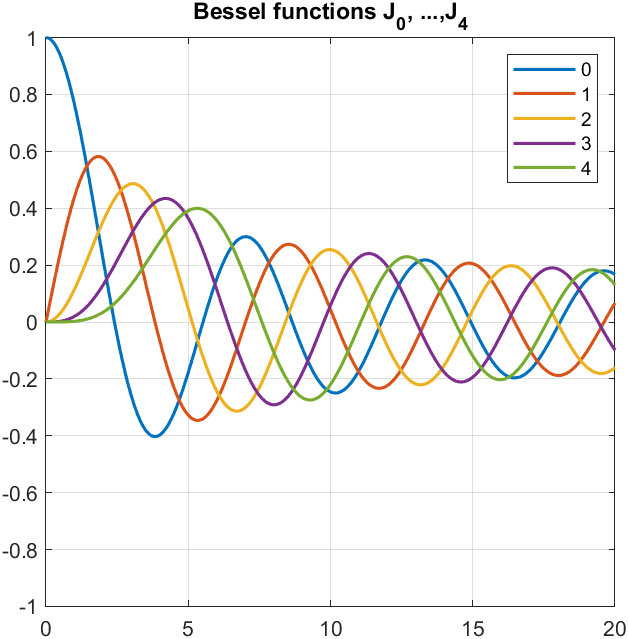
\includegraphics[width=.3\textwidth]{figs/besselj.png}\hfil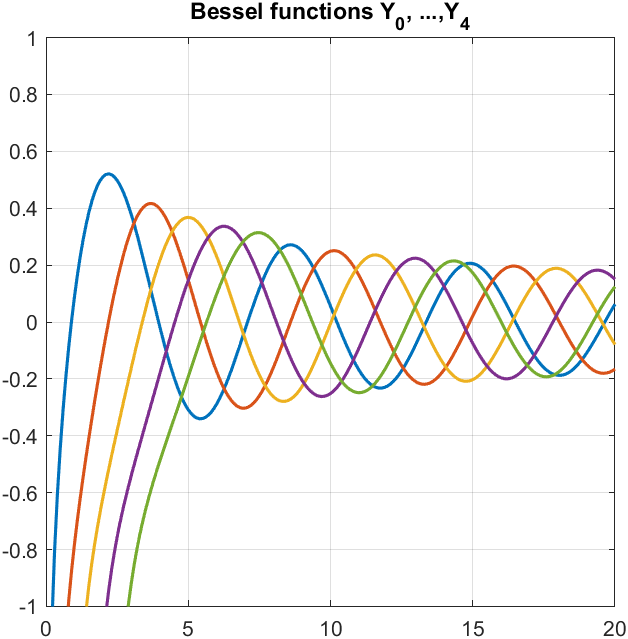
\includegraphics[width=.3\textwidth]{figs/bessely.png}\hfil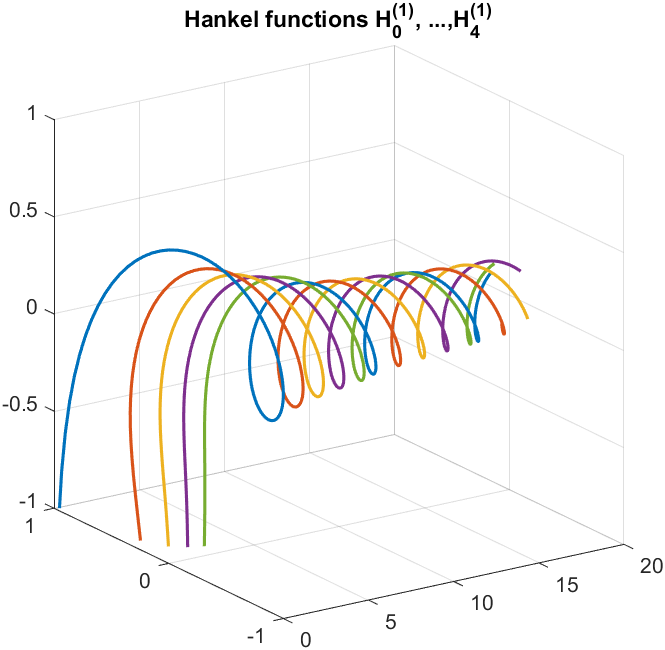
\includegraphics[width=.3\textwidth]{figs/hankel.png}
		\end{figure}
		\end{small}
	\end{frame}
	
	\begin{frame}{Soluzioni particolari dell'equazione di Helmholtz}
		\begin{small}
			\begin{block}{Onde circolari}
			Le funzioni della forma $J_\ell(kr)\re^{\ri \ell \theta}$ e $Y_\ell(kr)\re^{\ri \ell \theta}$ sono soluzioni dell'equazione di Helmoltz e sono dette \textbf{onde circolari} o funzioni di \textbf{Fourier-Bessel}. Un caso speciale sono le funzioni di \textbf{Fourier-Hankel} $H^{(1)}_\ell(kr)\re^{\ri \ell \theta}$ e $H^{(2)}_\ell(kr)\re^{\ri \ell \theta}$.
		\end{block}
		\begin{figure}
			\centering
			\hspace{-0.3cm}\animategraphics[loop,width=.55\textwidth]{10}{gif/c4b8918d-12ca-4be4-a91b-86ad45ca5061-}{0}{29}
			\caption{Parte reale di un'onda centrata $\bx_0 = (-1, 1)$}
		\end{figure}
		\end{small}
	\end{frame}
	
	\section{Multiple scattering}
	\sectionpage
	
	\begin{frame}{Onde contro gli ostacoli}
		\begin{small}
			Consideriamo un'onda che colpisce un ostacolo impenetrabile $D \subset \IR^2$; possiamo imporre diverse condizioni su $\partial D$:
			\begin{columns}
				\begin{column}{0.6\textwidth}
					\begin{block}{}
						\begin{itemize}
							\item Se l'ostacolo è \textbf{sound-soft}, imponiamo una condizione di Dirichlet: $u=0$;
							\item Se l'ostacolo è \textbf{sound-hard}, imponiamo una condizione di Neummann: $\frac{\partial u}{\partial \bn}=0$;
							\item Possiamo imporre anche una condizione di \textbf{impedenza}: $\frac{\partial u}{\partial \bn} - \ri k u=0$.
						\end{itemize}
					\end{block}
	
				\end{column}
				\begin{column}{0.4\textwidth}
					\begin{center}
						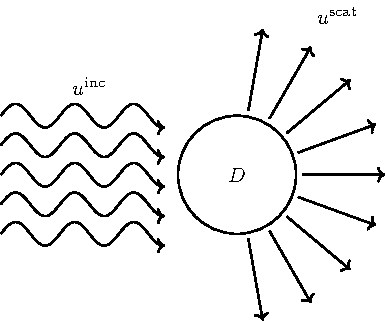
\includegraphics[width=\textwidth]{figs/scat.pdf}      
					\end{center}
				\end{column}
			\end{columns}
			\vspace*{0.5cm}
			Generalmente si differenziano l'\textbf{onda incidente} $u^\inc$ e l'\textbf{onda riflessa} $u^\scat$ e si scrive $u=u^\tot=u^\inc+u^\scat$.		
		\end{small}
	\end{frame}
	
	\begin{frame}{Scattering Problem}
		\begin{small}
			Data un'onda incidente $u^\inc$ e un ostacolo $D\subset \IR^2$, voglio trovare $u = u^\inc + u^\scat$ \\che soddisfi l'equazione di Helmholtz in $\IR^2 \setminus D$ e una condizione al bordo su $\partial D$.
		
		Per trovare un'unica soluzione $u$, dobbiamo anche imporre una condizione all'infinito
		\begin{block}{Sommerfeld Radiation Condition}
			Diciamo che $u$ soddisfa la \textbf{condizione di radiazione di Sommerfeld (SRC)} se
			\begin{equation*}
				\bigg|\frac{\partial u^\scat}{\partial r} - \ri ku^\scat\bigg| = o(r^{-1/2}), \qquad r \to \infty
			\end{equation*}
			uniformemente in tutte le direzioni.
		\end{block}
		Si ottiene il seguente problema
		\begin{equation*}
			\begin{cases}
				\Delta u + k^2 u = 0 & \text{in} \,\, \IR^2 \setminus D, \\
				u = 0 \left( \frac{\partial u}{\partial \bn}=0 \right) & \text{su} \,\, \partial D, \\
				\text{SRC} & r \to \infty.
			\end{cases}
		\end{equation*}
		\end{small}
	\end{frame}
	
	\begin{frame}{Sulla condizione di radiazione}
		\begin{small}
		\begin{block}{}
			Dal punto di vista fisico la condizione di radiazione equivale a chiedere che l'onda scatterata \textbf{si allontani} dall'ostacolo all'infinito.
		\end{block}
		
		Guardando le funzioni di Bessel e Hankel, osserviamo che per $r\to\infty$
		\begin{align*}
			& J_\ell(r) \sim \sqrt{\frac{2}{\pi r}} \cos(r - \phi_\ell), & & Y_\ell(r) \sim \sqrt{\frac{2}{\pi r}} \sin(r - \phi_\ell), \\
			& H_\ell^{(1)}(r) \sim \sqrt{\frac{2}{\pi r}}  \re^{\ri (r - \phi_\ell)}, & & H_\ell^{(2)}(r) \sim \sqrt{\frac{2}{\pi r}}  \re^{-\ri (r - \phi_\ell)},
		\end{align*}
		dove $\phi_\ell := \frac{\ell \pi}{2}+\frac{\pi}{4}$.
		
		Quindi, se vogliamo considerare delle onde \textbf{"uscenti"}, selezioneremo le $H_\ell^{(1)}(r)$.
		\end{small}
	\end{frame}
	
	\begin{frame}{Multiple Scattering Problem}
		\begin{small}
			\begin{columns}
				\begin{column}{0.5\textwidth}
					\begin{block}{}
						Dato $N\in\IN$, consideriamo il problema di un'onda che si riflette contro $N$ ostacoli sound-soft $D_j \subset \IR^2$, con $j = 1,\cdot\cdot\cdot,N$, e chiamiamo $D:=D_1 \cup D_2 \cup \cdot\cdot\cdot \cup D_N$.
					\end{block}
				\end{column}
				\begin{column}{0.4\textwidth}
					\begin{center}
						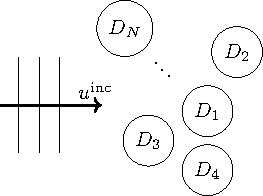
\includegraphics[width=\textwidth]{figs/multiple.pdf}      
					\end{center}
				\end{column}
			\end{columns}
			\vspace*{0.4cm}
			Vogliamo risolvere
			\begin{equation*}
				\begin{cases}
					\Delta u + k^2 u = 0 & \text{in} \,\, \IR^2 \setminus D, \\
					u = 0  & \text{su} \,\, \partial D, \\
					\text{SRC} & r \to \infty.
				\end{cases}
			\end{equation*}
		\end{small}
	\end{frame}
	
	\begin{frame}{Risoluzione del problema - Primo approccio}
		Dato che ho un numero limitato di ostacoli, $\exists R>0$ tale che $D \subset B_R(0)$. quindi posso risolvere il problema su un insieme finito e utilizzare tecniche classiche come per esempio gli elementi finiti.
		\begin{figure}
			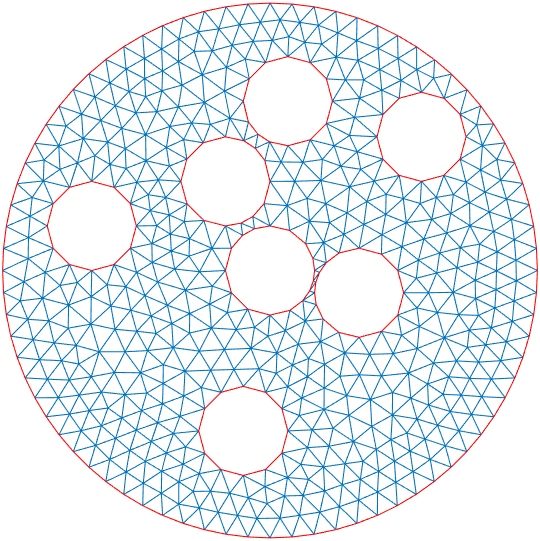
\includegraphics[width=0.3\textwidth]{figs/mesh.png}
		\end{figure}
		\begin{block}{Problema}
			Questo approccio risulta molto \textbf{costoso} e \textbf{inefficiente}.
		\end{block}
	\end{frame}
	
	\section{Il metodo della T-matrix}
	\sectionpage
	
	\begin{frame}{Il caso di un solo ostacolo}
		
		\begin{columns}
			\begin{column}{0.4\textwidth}
				\begin{block}{}
					Ci concentriamo sul problema di scattering su un unico ostacolo sound-soft \textbf{circolare} di raggio $R>0$. Data un'onda incidente $u^\inc$, vogliamo trovare la soluzione $u=u^\tot$ del problema di scattering.
				\end{block}
			\end{column}
			\begin{column}{0.5\textwidth}
				\begin{center}
					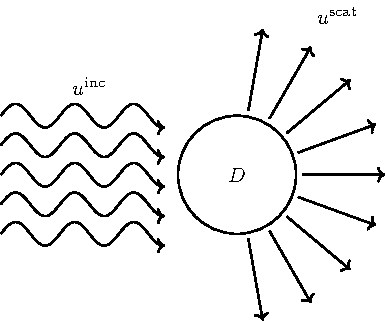
\includegraphics[width=\textwidth]{figs/scat.pdf}      
				\end{center}
			\end{column}
		\end{columns}
	\end{frame}
	
	\begin{frame}{Espansione in serie}
		\begin{block}{}
			Espandiamo in termini delle funzioni di Bessel e di Hankel:
			\begin{align*}
				& u^\inc(r,\theta)=\sum_{n \in \IZ} a_n J_n(kr)\re^{\ri n\theta}, \\
				& u^\scat(r,\theta)=\sum_{n \in \IZ} b_n H_n^{(1)}(kr)\re^{\ri n\theta},
			\end{align*}
			dove i coefficienti $a_n$ sono calcolati a partire da $u^\inc$, che è nota, mentre i coefficienti $b_n$ sono incogniti. L'espansione di $u^\scat$ ci permette di soddisfare automaticamente la condizione di radiazione.
		\end{block}
	\end{frame}
	
	\begin{frame}{La T-matrix}
		\begin{small}
			Applicando la condizione al bordo, ovvero che
		\begin{equation*}
			u^\tot(r,\theta)=u^\inc(r,\theta)+u^\scat(r,\theta)=0,
		\end{equation*}
		si ottiene la seguente equazione
		\begin{equation*}
			b_n = \sum_{m \in \IZ} \mathbf{T}_{n,m} a_m.
		\end{equation*}
		\begin{block}{}
			I coefficienti $\mathbf{T}_{m,n}$ costruiscono una matrice (infinita) che viene chiamata \textbf{T-matrix}, e che stabilisce la relazione tra i coefficienti dell'onda incidente $a_n$ e quelli dell'onda riflessa $b_n$. 
		\end{block}
		
		Per un ostacolo circolare, grazie all'ortogonalità delle $\re^{\ri n\theta}$, si ha che 
		\begin{equation*}
			\mathbf{T}_{n,m} = -\delta_{n,m} \frac{J_n(kR)}{H_n^{(1)}(kR)}.
		\end{equation*}
		\end{small}
	\end{frame}
	
	\begin{frame}{Calcolo della T-matrix nel caso generale}
		\begin{block}{}
			Se il mio ostacolo non è una sfera, calcolare la T-matrix richiede un'approssimazione numerica. Ci sono vari metodi per calcolarla:
			\begin{itemize}
				\item Utilizzare la forma integrale dell'equazione di Helmholtz;
				\item Risolvere l'equazione di Helmholtz per diversi campi incidenti (es., armoniche sferiche o onde piane), discretizzando la soluzione con un metodo appropiato (FEM, BEM, ecc.);
				\item Null Field Method o Extended Boundary Condition Method - EBCM.
			\end{itemize}
		\end{block}
	\end{frame}
	
	\begin{frame}{Utilizzo della T-matrix}
		\begin{block}{}
			\begin{itemize}
			\item Determino i coefficienti $a_n$ dell'espansione dell'onda incidente;
			\item Utilizzo la T-matrix per calcolare i coefficienti $b_n = \sum_{m \in \IZ} \mathbf{T}_{n,m} a_m$;
			\item Ricostruisco $u^\scat(r,\theta) = \sum_{n \in \IZ} b_n H_n^{(1)}(kr)\re^{\ri n\theta}$;
			\item Scrivo il campo totale come $u^\tot = u^\inc + u^\scat$.
		\end{itemize}
		\end{block}
		Il vantaggio della T-matrix è che dipende solo dalla \textbf{geometria dell'ostacolo} e non dall'onda incidente, quindi può essere utilizzata per studiare lo scattering di una varietà di onde incidenti.
	\end{frame}
	
	\begin{frame}{Esempio: onda piana incidente}
		Se $u^\inc(\bx) = \re^{\ri k \bx} = \re^{\ri k \cos \theta}$, espandendo in armoniche circolari $$u^\inc(r,\theta)=\sum_{n \in \IZ} \ri^n J_n(kr)\re^{\ri n\theta},$$ quindi otteniamo i coefficienti $a_n=\ri^n$.
		\begin{block}{}
			Possiamo ricostruire il campo scatterato come
			\begin{equation*}
				u^\scat(r,\theta) = - \sum_{n \in \IZ} \frac{J_n(kR)}{H_n^{(1)}(kR)} \ri^n H_n^{(1)}(kr) \re^{\ri n \theta}.
			\end{equation*}
		\end{block}
	\end{frame}
	
	\begin{frame}{Il caso di più ostacoli}
		\begin{small}
		Consideriamo $N$ ostacoli $D_j$, ciascuno con una sua T-matrix $\mathbf{T}_j$. 
		
		Per l'ostacolo $D_j$, il campo incidente totale è dato dalla somma tra $u^\inc$ e il campo scatterato dagli altri ostacoli. Possiamo scrivere
		\begin{equation*}
			\mathbf{a}_j = \mathbf{a}_j^\inc + \sum_{l \neq j} \mathcal{U}_{j,l} \mathbf{b}_l = \mathbf{a}_j^\inc + \sum_{l \neq j} \mathcal{U}_{j,l} \mathbf{T}_l \mathbf{a}_l,
		\end{equation*}
		dove $\mathbf{a}_j^\inc$ è il vettore dei coefficienti di $u^\inc$ sull'ostacolo $j$ e $\mathcal{U}_{j,l}$ è una matrice di traslazione. Si ottiene il seguente sistema a blocchi
		\begin{equation*}
			\left[\begin{matrix}
				\mathbf{I} & -\mathcal{U}_{1,2}^T \mathbf{T}_2 & \cdot\cdot\cdot & -\mathcal{U}_{1,N-1}^T \mathbf{T}_{N-1} & -\mathcal{U}_{1,N}^T \mathbf{T}_N\\
				-\mathcal{U}_{2,1}^T \mathbf{T}_1 & \mathbf{I} & -\mathcal{U}_{2,3}^T \mathbf{T}_3 & \cdot\cdot\cdot & -\mathcal{U}_{2,N}^T \mathbf{T}_N \\
				 & \vdots & & & \vdots \\
				-\mathcal{U}_{N,1}^T \mathbf{T}_1 & \cdot\cdot\cdot & \cdot\cdot\cdot & -\mathcal{U}_{N,N-1}^T \mathbf{T}_{N-1} & \mathbf{I}
			\end{matrix}\right] \left[ \begin{matrix}
			\mathbf{a}_1 \\ \mathbf{a}_2 \\ \vdots \\ a_N
			\end{matrix} \right] = \left[ \begin{matrix}
			\mathbf{b}_1 \\ \mathbf{b}_2 \\ \vdots \\ b_N
			\end{matrix} \right]
		\end{equation*}
		\end{small}
	\end{frame}
	
	\begin{frame}{Considerazioni sulla T-matrix}
		\begin{block}{}
			\begin{itemize}
				\item Siccome $\mathbf{T}$ è una matrice infinita, dovrò approssimarla con una matrice finita. L'ordine di approssimazione dipende dal numero d'onda e dalle dimensioni degli ostacoli;
				\item  Posso calcolare la T-matrix di diversi ostacoli in contemporanea, riducendo i tempi computazionali;
				\item Una volta costruite le T-matrix, posso risolvere il problema per qualsiasi onda incidente, senza dovermi costruire ogni volta tutto;
				\item Per calcolare effettivamente la T-matrix esistono dei software come \textrm{TMATROM} su MATLAB o \textrm{MultipleScattering} su Julia.
			\end{itemize}
		\end{block}
	\end{frame}
	
	\begin{frame}{Esempio: random scattering}
		\begin{small}
		\begin{block}{}
			Consideriamo $N=70$ ostacoli circolari di raggio $0.1$ generati casualmente sul rettangolo $[0,5] \times [-5,5]$ e un'onda piana incidente con direzione $\bd=(\sqrt{3}/2, 1/2)$.
			
			I risultati sono stati ottenuti con il pacchetto \textrm{MultipleScattering} di Julia.
		\end{block} 
		\begin{figure}
			\animategraphics[loop,width=.65\textwidth]{10}{gif/4430fed9-5958-4984-83b6-1bb0365d34fc-}{0}{29}
		\end{figure}
		\end{small}
	\end{frame}
	
	\section{La gabbia di Faraday}
	\sectionpage
	
	\begin{frame}{Che cos'è la gabbia di Faraday?}
		\begin{center}
			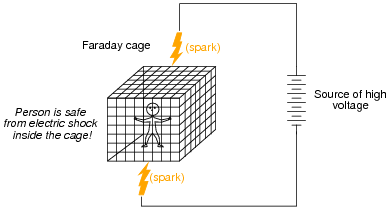
\includegraphics[width=.5\textwidth]{figs/cage.png}      
		\end{center}
		La \textbf{gabbia di Faraday} è un dispositivo che blocca i campi elettrici esterni, proteggendo il suo interno da interferenze elettrostatiche. 
		
		La gabbia è costituita da un involucro conduttore, che può essere realizzato con materiali come rame, alluminio o acciaio, e può avere una struttura piena o reticolata (ad esempio una rete metallica).
	\end{frame}
	
	\begin{frame}{Gabbia di Faraday per Helmholtz}
		\begin{columns}
			\begin{column}{.6\textwidth}
				Il caso 2D può essere visto come una sezione trasversale di quello 3D. In questo caso $u$ rappresenta la componente del campo elettrico esterna al piano e soddisfa l'equazione di Helmholtz $\Delta u + k^2 u = 0$.
				
				Ogni punto nero è la sezione di un filo infinito, e la condizione al contorno è $u=0$ su tutti i dischi.
			\end{column}
			\begin{column}{.4\textwidth}
				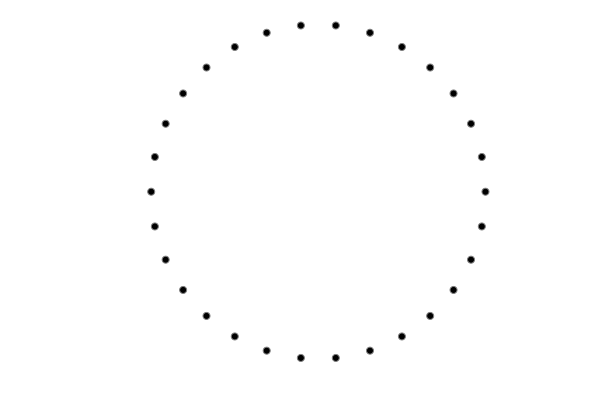
\includegraphics[width=\textwidth]{figs/wire.png}
			\end{column}
		\end{columns}
		\vspace*{0.3cm}
		\begin{block}{}
			Possiamo trattare lo studio della gabbia di Faraday come un problema di \textbf{multiple scattering}.
		\end{block}
	\end{frame}
	
	\begin{frame}{Problema modello}
			\begin{columns}
			\begin{column}{.6\textwidth}
				Consideriamo una circonferenza di raggio $R=1$ e una gabbia composta da $N=30$ cerchietti equidistanti di raggio $r=0.02$. 
			\end{column}
			\begin{column}{.3\textwidth}
				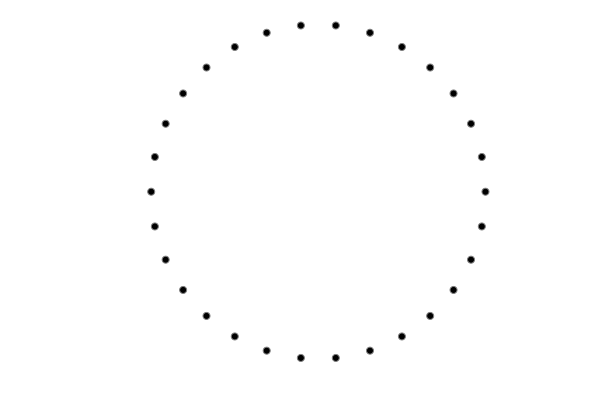
\includegraphics[width=\textwidth]{figs/wire.png}
			\end{column}
		\end{columns}
		Scegliamo come onda incidente un'onda circolare $$u^\inc = H_0^{(1)}(|\bx - \bx_0|)$$ centrata in $\bx_0=(2,0)$.
%		\vspace*{0.4cm}
%		Si può verificare che nell'origine il campo totale è approssimato da
%		\begin{equation*}
%			u(0) \sim C \frac{i}{4}H_0^{(1)}(k|\bx_0|)\left(\frac{H_1^{(1)}(k)}{H_0^{(1)}(k)} - \frac{J_1^{(1)}(k)}{J_0^{(1)}(k)}\right), \qquad C \in \IR_+.
%		\end{equation*}
	\end{frame}
	
	\begin{frame}{Soluzione al variare di $k$}
		\begin{figure}
			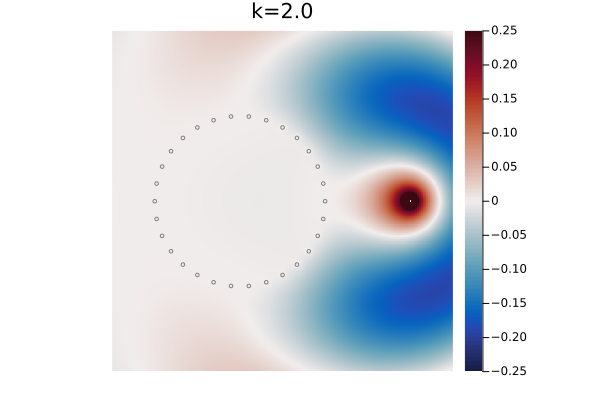
\includegraphics[width=.48\textwidth]{figs/resonant_plot_1.png}\hfil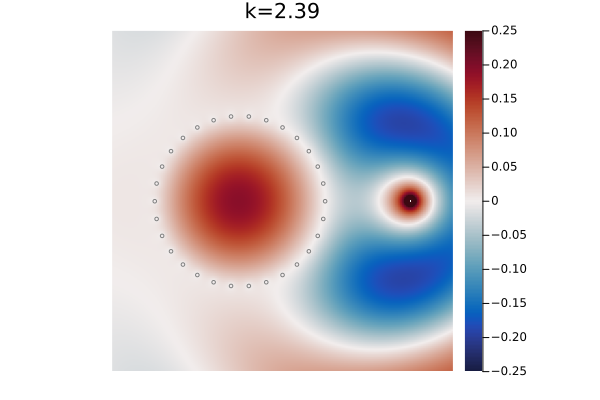
\includegraphics[width=.48\textwidth]{figs/resonant_plot_2.png}
			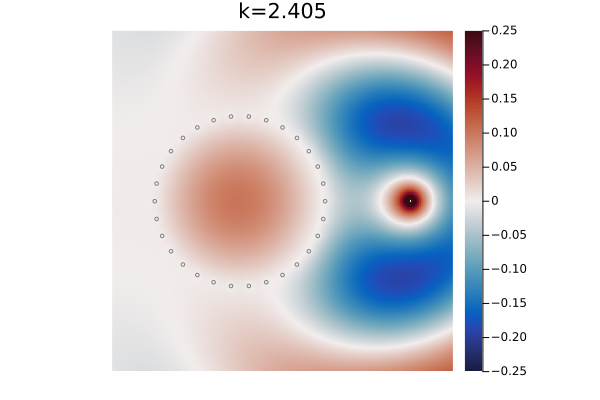
\includegraphics[width=.48\textwidth]{figs/resonant_plot_3.png}\hfil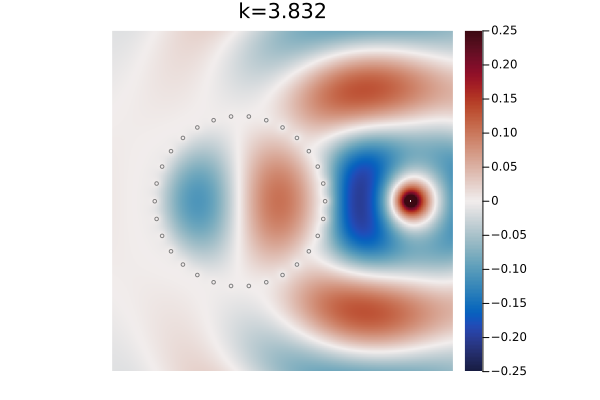
\includegraphics[width=.48\textwidth]{figs/resonant_plot_4.png}
		\end{figure}
	\end{frame}
	
%	\begin{frame}{Differenti comportamenti della gabbia di Faraday}
%		\begin{figure}
%			\animategraphics[loop,width=.5\textwidth]{10}{gif/04c2d196-4c11-41f4-971d-605a51bdb428-}{0}{29}\animategraphics[loop,width=.5\textwidth]{10}{gif/e651c9c7-72e6-40d4-a4ff-9ef196f1da22-}{0}{29}
%		\end{figure}
%	\end{frame}
	
	\begin{frame}{Il fenomeno della risonanza}
		\begin{block}{}
			Per alcuni valori di $k$ la gabbia fallisce e anzi amplifica l'ampiezza dell'onda: questo è il fenomeno della \textbf{risonanza}.
		\end{block}	
		\vspace*{0.3cm}
		La risonanza si verifica quando scegliamo un numero d'onda tale che $k^2$ sia \textbf{autovalore del Laplaciano} sul cerchio.
		
		Le onde si riflettono continuamente all'interno della gabbia e interferiscono, generando modi stazionari. 
		
		Per il cerchio di raggio $1$, questi valori di $k$ corrispondono agli zeri delle funzioni di Bessel $J_\ell$.
	\end{frame}
	
	\begin{frame}{Esempio: risonanza per lo zero di $J_3$}
		\begin{small}
		\begin{block}{}
			Scegliamo $k^*$ tale che $J_3(k^*)=0$; si trova numericamente che $k^*=6.3801618959$.
			
			Risolvendo il problema per questo specifico numero d'onda, siamo in grado di ricreare la risonanza all'interno della gabbia di Faraday.
		\end{block}
		\begin{figure}
			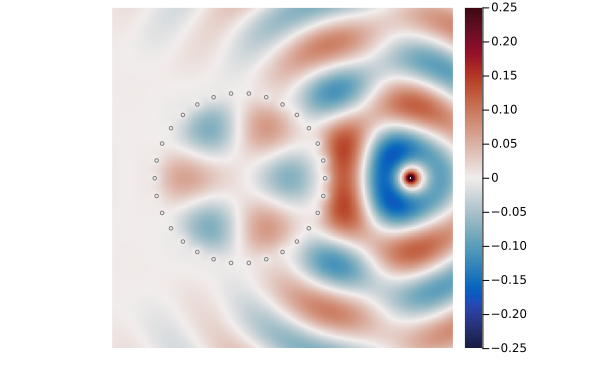
\includegraphics[width=.48\textwidth]{figs/resonant_plot_5.png}\hfil\animategraphics[loop,width=.46\textwidth]{10}{gif/69698602-dc04-4783-bc11-5850e06163cc-}{0}{29}
		\end{figure}	
		\end{small}
	\end{frame}
	
	\begin{frame}{Un esempio interessante}
		\begin{columns}
			\begin{column}{.5\textwidth}
				\begin{block}{}
					Consideriamo due gabbie composta da $N=30$ cerchietti equidistanti di raggio $r=0.02$ disposte come in figura. La gabbia centrata nell'origine ha raggio $R_1 = 1$, mentre l'altra ha raggio $R_2=0.9$. Consideriamo un'onda piana incidente centrata in $\bx_0$. Cosa succede se scegliamo $k$ in modo da avere risonanza nella prima gabbia?
				\end{block}
			\end{column}
			\begin{column}{.5\textwidth}
				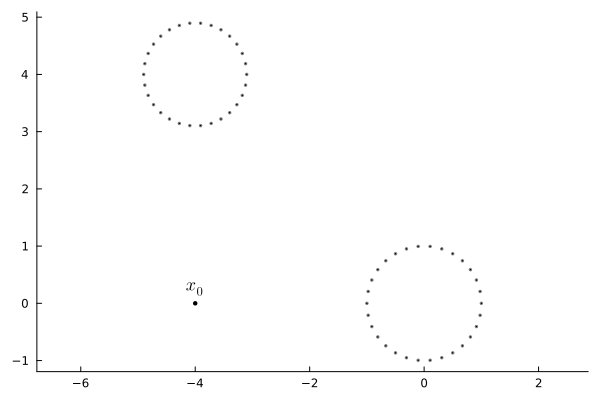
\includegraphics[width=\textwidth]{figs/domain.png}
			\end{column}
		\end{columns}
	\end{frame}
	
	\begin{frame}{Risultati}
		\begin{figure}
			\animategraphics[loop,width=.5\textwidth]{10}{gif/db831154-8b0c-4d5c-994c-ebb9142dd427-}{0}{29}\animategraphics[loop,width=.5\textwidth]{10}{gif/8fdc3e46-7f8c-4188-a9dd-f999098b51ab-}{0}{29}
			\caption{Risultati per $k=2.39$ e $k=3.832$.}
		\end{figure}
	\end{frame}
	
	\begin{frame}{References}		
		\begin{thebibliography}{10}
			\bibitem{d}{P. A. Martin}
			\newblock {Multiple scattering; Interaction of time-harmonic waves with N obstacles}
			\newblock {Encyclopedia of Mathematics and its application(1995)}.
			
			\bibitem{c}{A. L. Gower et al.}
			\newblock {Reflection from a multi-species material and its transmitted effective wavenumber}
			\newblock {Proc. R. Soc. A.474 (2018)}.
			
			\bibitem{a}{D. P. Hewett and I. J. Hewitt}
			\newblock  {Homogenized boundary conditions and resonance effects in Faraday cages}
			\newblock {Proc. R. Soc. A.472 (2016)}.
			
			\bibitem{b}{L. N. Trefethen}
			\newblock {Surprises of the Faraday cage}
			\newblock {SIAM News 49 (2016)}.
		\end{thebibliography}
	\end{frame}
	
	\section*{Grazie per l'attenzione!}
	\sectionpage
	
\end{document}